\chapter{Extraction of spin correlation}

\section{Likelihood Fit}
\label{sec:extraction}

The amount of spin correlation observed in the data is extracted using a binned maximum likelihood method. Two templates are constructed; one with SM \ttbar\ spin correlations and one with no included \ttbar\ spin correlation. The templates are fit to the data and the degree to which the data fits the SM case is extracted ($f_{SM}$). The cross section of the two \ttbar\ templates taken together is also extracted. 

The likelihood function may be written as:

\begin{equation}
  \begin{aligned}
    =-ln(L) = \mathcal{L} = \displaystyle\sum\limits_{n=0}^{N} Data*\ln\{B + n_{tt}(f_{SM}*S + (1-f_{SM})*NS)\} \\
                  - (B + n_{tt}(f_{SM}*S + (1-f_{SM})*NS) \\
		  - \ln(Data!) \\
  \end{aligned}
\end{equation}

Where $Data$ is the measured number of data events, $S$ is the estimated number of events in the spin sample, $NS$ is the estimated number of events in the uncorrelated sample, $N$ is the number of bins, $n_{tt}$ is the normalisation of the \ttbar\ templates and $B$ is the background estimate. This likelihood function is minimised as function of $f_{SM}$ and the \ttbar\ cross section. The cross section is allowed to vary in order to reduce the influence of normalization uncertainties on the result of $f_{SM}$. For the maximization procedure we use the SIMPLEX and MIGRAD algorithms in the TMinuit package~\cite{James:1975dr}.

The fitting method was validated using a linearity check. The templates were mixed to create pseudo-data sets of simulated spin correlation in the range $f_{SM} = -1 \rightarrow +2$ and the spin correlation extracted. The result is shown in Fig.~\ref{fig:linearity}. No bias is observed in the extraction procedure in the quoted range.

Since each analysis channel is orthogonal, due to the lepton flavour selection, we may multiply the likelihoods to perform a multi channel fit. 

\begin{figure}[h!]
	\begin{center}
	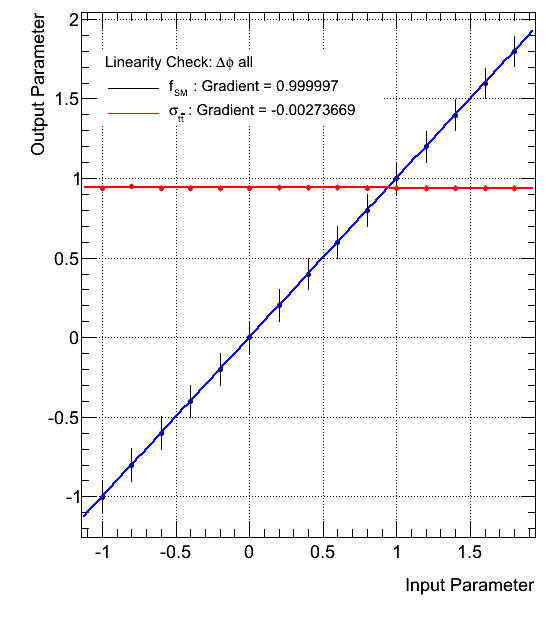
\includegraphics[width=85mm]{f/delta_phi10all_syst_linLinearity}
	\end{center}
	\caption{Linearity check comparing different values of input $f_{SM}$ or \ttbar\ cross section to those extracted by the fit.}
	\label{fig:linearity}
\end{figure}

\section{Systematic Uncertainties}
\label{sec:systematics}

%The use of Monte Carlo simulations in this analysis presents an inherent problem. Though the degree to which these samples accurately reflect the true physics processes that they simulate is impressive, they are not perfect. A systemic disparity occurs between our assumption ( the rates and shapes of the signal and backgrounds distributions ) and the observed data. This is described as a ``systematic'' uncertainty. The effect of these systematic uncertainties, or more simply put the effect of the difference between our simulation and truth, must be quantified. In addition, systematic uncertainties can arrise from effects such as detector modelling, or data driven background estimation techniques and these must also be accounted for. 

The degree to which the systematic uncertainty effects the result is quoted within a 68\% confidence interval (1$\sigma$ deviation) by convention. Ensemble tests are used to estimate the effect of a source of uncertainty. New templates are generated with an estimated 1$\sigma$ shift in the source of uncertainty for both the spin correlated template (spin) and the uncorrelated (no-spin) template.  
Pseudo-data sets are generated by mixing these templates to the observed $f_{SM}$ and Poisson fluctuating their bin content.
The nominal templates are then fitted to the pseudo-data. In addition, the systematic shifted templates are simultaneously fitted to the same pseudo-data and the difference between the two fits are then saved. This procedure is performed 1000 times for each systematic, and the final uncertainty is quoted as the mean of the difference between the two fits.
	The motivation for simultaneously fitting the shifted and the nominal templates to the pseudo-data is to remove statistical fluctuations in the fit. When fitting the shifted templates to the pseudo-data (that has been created from these templates), any deviation from the input spin correlation will be caused by statistical fluctuations in creating the pseudo-data, and will be identical when the nominal templates are fitted to this pseudo-data. By taking the difference between both fits we remove this statistical fluctuation. The step by step procedure for the fitting is summarised below:
 
\begin{enumerate}
	\item Fit the nominal templates $\mathbf{T}_{spin}$, $\mathbf{T}_{nospin}$ to the data $\mathbf{D}$ and obtain $f_{SM}^{nominal}$.
	\item Generate new spin and no spin templates, with a systematic shift \textbf{X} included, $\mathbf{T}^{\mathbf{X}}_{spin}$, $\mathbf{T}^{\mathbf{X}}_{nospin}$.
	\item Construct pseudo data $\mathbf{D^\prime}$ by mixing $\mathbf{T}^{\mathbf{X}}_{spin}$ and $\mathbf{T}^{\mathbf{X}}_{nospin}$ to the observed $f_{SM}^{nominal}$. 
        \item Poisson vary each bin in $\mathbf{D^\prime}$, using the bin content as the mean.
	\item Fit $\mathbf{T}_{spin}$, $\mathbf{T}_{nospin}$ to $\mathbf{D^\prime}$ and obtain $f_{SM}^{\prime}$.
	\item Fit $\mathbf{T}^{\mathbf{X}}_{spin}$, $\mathbf{T}^{\mathbf{X}}_{nospin}$ to $\mathbf{D^\prime}$ and obtain $f_{SM}^{\mathbf{X}}$.
	\item Take the difference $f_{SM}^{\mathbf{X}}$ - $f_{SM}^{\prime}$
	\item Repeat steps 3 $\rightarrow$ 6 1000 times.
	\item Take $<f_{SM}^{\mathbf{X}}$ - $f_{SM}^{\prime}>$ as the systematic uncertainty due to \textbf{X} .
\end{enumerate}

%\begin{figure}[htbp]
%\begin{center}
%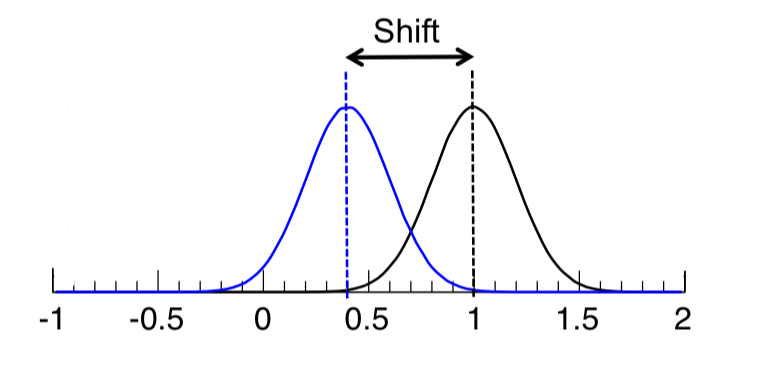
\includegraphics[width=100mm]{f/GaussianFigure}
%\end{center}
%\caption{Illustration of systematic estimation procedure. The caussian curve generated by the systemati shifted pseudo experiments is showin in blue, the nominal fit is shown in black}
%\label{fig:syst_gaussian}
%\end{figure}

Each source of systematic uncertainty is assumed to be uncorrelated and for the total systematic uncertainty all of the individual sources are added in quadrature. We give an overview over all sources of systematic uncertainties that we consider and the methods by which they are estimated. For simplicity we categorise systematic uncertainties into two types: 
\begin{itemize}
	\item ``Normalisation uncertainties'': which only effect the rate of a particular background or signal sample.
	\item ``Shape changing systematics'': which effect the shape of the variable of interest, in addition to its normalisation. 
\end{itemize}
Normalisation uncertainties typically have a small effect on the extracted spin correlation as the normalisation of the signal templates is allowed to float in the likelihood fit ( i.e. the floating of the \ttbar\ cross section described in section \ref{sec:extraction}. Shape changing uncertainties are the dominant form of uncertainty in the analysis and can have a marked impact on the spin correlation.

\vspace{5mm}
\noindent
\textbf{Luminosity:}
\begin{itemize} 
     \item For data taken in the 7 TeV LHC running period, the Luminosity uncertainty is taken to be a flat uncertainty of $\pm1.8$~\% on the normalisation of the data, established primarily through Van-De-Meer scans performed during data taking, and comparisons with the CMS detector. The systematic uncertainty is estimated by varying the normalisation of both the signal and background samples simultaneously, up and down by this value.
\end{itemize}

\vspace{5mm}
\noindent
\textbf{Electrons:}
\begin{itemize}
    \item Energy Scale: All electrons are corrected for electron energy scale by default in the Monte Carlo. To estimate the systematic uncertainty this energy scale is shifted by $\pm 1\sigma$ of the uncertainty from the energy scale estimation procedure, in addition to the default scaling. 
    \item Trigger Scale Factor: To estimate the uncertainty on the scale factor associated with trigger modelling, the scale factors are varied by $\pm 1\sigma$~ from the default scale factor.
    \item Energy Resolution: The Monte Carlo is smeared by default to correct for the difference in the modelling of electron energy resolution with the data. Additional smearing is performed to estimate the uncertainty.
\end{itemize}

\vspace{5mm}
\noindent
\textbf{Muons:}
\begin{itemize}
    \item Momentum Shift: There are two possible sources of muon momentum uncertainty, those from the muon spectrometer (MS) and those from the inner detector (ID). The muon momentum is shifted by $\pm~1~\sigma$ in the MS and ID independently. The largest and smallest shift are averaged to provide the uncertainty. Correlations between these parameters are accounted for.
    \item Resolution: The Monte Carlo is smeared by default to correct for the difference in energy resolution with the data. Additional smearing is performed to estimate the uncertainty.
    \item Momentum Scale: To estimate the effect of muon momentum scaling in the MC, this is disabled and the fit re-performed. The result is then symmetrised and taken as the systematic shift.
\end{itemize}

\vspace{5mm}
\noindent
\textbf{Jets:}
Jets represent one of the most difficult physical objects to model correctly in Monte Carlo and as such have a large number of sources of systematic uncertainty. 
\begin{itemize}
    \item Jet Energy Scale (JES): A total of 61 sources of systematic uncertainty exist in relation to JES. Fortunately, many of these are correlated and it is possible to fully cover the uncertainty using 21 uncorrelated variations.
%	\begin{enumerate}
%	\item JES Component 1
%	\item JES Component 2
%	\item JES Component 3
%	\item JES Component 4
%	\item JES Component 5
%	\item JES Component 7
%	\item JES Component 8
%	\item JES Component 9	
%	\item JES Component 10
%	\item JES Component 11	
%	\item JES Component 12
%	\item JES Component 13	
%	\item \textit{Flavour Response} - Uncertainty associated with the flavour composition of each jet.
%	\item \textit{B-JES} - Energy scale associated with jets tagged with b flavour.
%	\end{enumerate}	
    \item Energy Resolution: Jet energies are smeared within uncertainties derived from resolution measurements over the full 2011 data set. 
    \item Reconstruction Efficiency: The efficiency to reconstruct jets is not 100\% and not identical between data and Monte Carlo. In order to estimate the effect of this efficiency, jets are randomly dropped from the nominal sample and the spin correlation is re-extracted within an efficiency range derived from data. The shift between this sample and the nominal is symmetrised and taken as the uncertainty.
\end{itemize}

\vspace{5mm}
\noindent
\textbf{MET:}
\begin{itemize}
    \item Pileup: In order to estimate the effect of pileup on MET, the values for MET are scaled up and down by a 6.6\% uncertainty. 
    \item Soft Jet - Cell Out Correction: The systematics due to energy in calorimeter cells not associated to a physics object ('Cell out') and soft jets used in the calculation of the missing ET are 100\% correlated and evaluated together. 
\end{itemize}

\vspace{5mm} 
\noindent
\textbf{Generator Uncertainties:}\\
 Uncertainties due to features of the various MC generators are difficult to estimate. In most cases, the source of uncertainty is not sufficiently understood to investigate the effect at one confidence level, with the trivial exception of template statistics. We therefore estimate these uncertainties with the understanding that in most cases, there could be an over-estimation in the source of systematic uncertainty.% and quote them separately to the 1 $\sigma$ uncertainties.
 
\begin{itemize}
    \item Choice of Generator: Two generators are available at ATLAS to simulate \ttbar\ events at next to leading order, MC@NLO and POWHEG. The uncertainty on the choice of generator is estimated by performing the fit for both, with the difference taken as an uncertainty. In order to isolate only the Matrix element differences, both are interfaced to HERWIG to perform showering. Due to a bug in the POWHEG implementation the spin correlation was not included correctly and therefore this source of uncertainty would be significantly overestimated. Extracting the spin correlation directly from truth level in MC@NLO results in A=0.41 for the Maximal basis, in agreement with the SM prediction, whereas for POWHEG this results in A=0.33. This can be seen directly in Fig.~\ref{fig:generator_comparison}. For this reason, the systematics due to choice of generator was not included in the final systematics. Instead an uncertainty due to the choice of factorisation and renormalisation is used.

\begin{figure}[h]
	\begin{center}
	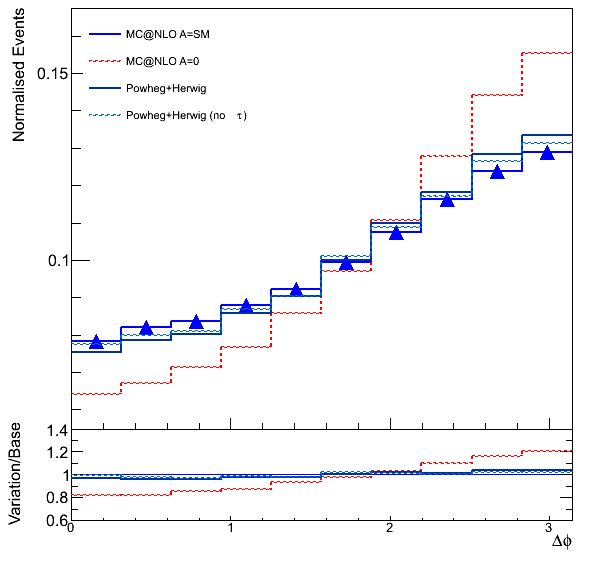
\includegraphics[width = 100mm]{f/truth_delta_Phi10generator_comparison}
	\end{center}
        \caption{Comparison between MC@NLO and POWHEG generators at truth level. POWHEG appears to be less correlated than the SM MC@NLO sample due to a POWHEG bug.}
        \label{fig:generator_comparison}
\end{figure}

    \item Scale choice: To estimate the effect of the choice of factorisation and renormalisation scales, samples are generated in which these scales are increased by a factor of two and reduced by a factor of a half.% It should be noted that this does not correspond to a 1 $\sigma$ experimental uncertainty and cannot be quoted as such. %Therefore this number is quoted as the theoretical uncertainty on the prediction from MC@NLO for A as this is an accepted method of estimating a theoretical uncertainty. 

    \item Parton Shower / Fragmentation model: The uncertainty due to the choice of the shower model is estimated by comparing POWHEG samples interfaced to HERWIG and the same POWHEG sample interfaced to PYTHIA. The POWHEG + HERWIG implementation suffered from the inclusion of unpolarised tau lepton decay, decreasing the spin correlation in this sample. In order to safely compare the HERWIG shower to the PYTHIA shower (which does not have this unpolarisation effect) we reject all dilepton events with tau decays at truth level. Spin correlation is also simulated incorrectly in these samples however we take the difference between the fits of the two samples as our uncertainty, mitigating this effect.

    \item ISR / FSR: The effect of initial state and final state radiation is estimated by taking two ACER MC samples, with the same matrix elements, and interfacing them with PYTHIA to perform showering. The amount of showering is scaled up and down to simulate more initial and final state radiation simultaneously. An analysis sensitive to jet radiation modelling determined that this procedure dramatically overestimated the observed jet radiation in data. %\ref{jetveto} .
 To compensate the systematic shift is taken as the difference between the two samples, scaled down by a factor of 2.

    \item Colour Reconnection: The effect of colour reconnection applied in MC is estimated by comparing two POWHEG \ttbar\ samples with different tunes for colour reconnection, the nominal colour reconnection and no colour reconnection. 

    \item Underlying event: The effect of underlying event modelling is estimated by comparing two POWHEG \ttbar\ samples each with different tunes for the underlying event model.

    \item Template Statistics: The effect of limited template statistics in the signal MC is estimated by Poisson fluctuating the standard model template by the number of weighted entries in each bin (as opposed to the nominal statistical uncertainty where the bins are Poisson fluctuated by the number of data entries in each bin). The result is then fitted to the original templates to obtain the systematic shift. 

\end{itemize}

\vspace{5mm}
\noindent
\textbf{PDF:}\\
In order to investigate the effect of the choice of PDF used in the analysis the analysis is repeated with different PDF sets. We consider our nominal PDF set (CTEQ10) and compare to NNPDF2.3 and MSTW2008nlo68cl. Each PDF set provides uncertainties due to the fit and the effect of these are evaluated at the 1 $\sigma$ level.
\begin{itemize}
  \item Intra PDF Uncertainty: Each PDF set considered has an associated number of systematic shifts due to various sources provided by the various PDF collaborations. The analysis is repeated with the templates reweighted to these shifted PDF values and the $f_{SM}$ extracted. An uncertainty band is calculated based on the recommendations of each PDF group. CTEQ uses an symmetric hessian method, NNPDF uses a root mean squared, and MSTW2008 uses an asymmetric hessian. The uncertainty in each PDF set is shown as a colour coded band in Fig.~\ref{fig:pdf}.
  \item Inter PDF Uncertainty: To calculate the overall effect of the choice of PDF set, and the uncertainties in each PDF set we use an envelope method. The uncertainty is taken to be the largest intra-pdf uncertainty from the central $f_{SM}$ value. This is illustrated in Fig.~\ref{fig:pdf}.
\end{itemize}

\begin{figure}[h]
	\begin{center}
	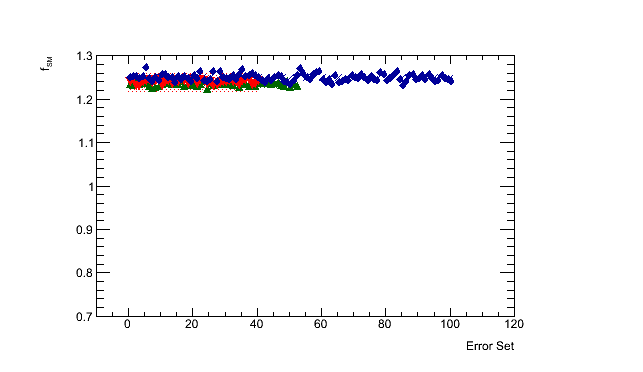
\includegraphics[width = 75mm]{f/delta_phi10emu_pdf_fsm}
	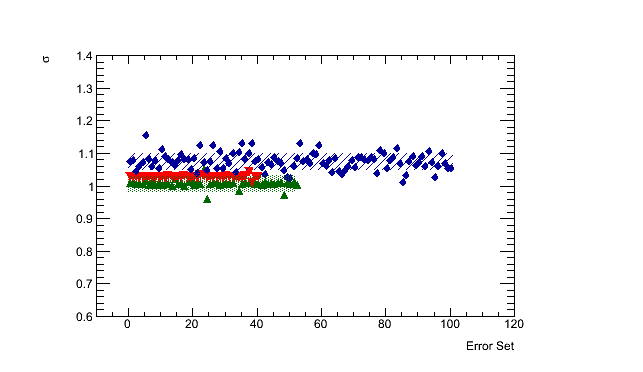
\includegraphics[width = 75mm]{f/delta_phi10emu_pdf_xsec}
	\end{center}
        \caption{Illustration of PDF uncertainties in the \emu channel for the extracted $f_{SM}$ \emph{(left)} and cross section \emph{(right)}. Each pdf set is colour coded such that NNPDF2.3 errors are shown in blue, CTEQ10 is shown in green and MSTW2008nlo68cl is shown in red.}
        \label{fig:pdf}
\end{figure}

\vspace{5mm}

\noindent
\textbf{Fake Leptons:}\\
The uncertainty due to mis-identified leptons is different depending on lepton flavour, and so each are measured separately (and combined in quadrature in the case of the \emu channel). 

\begin{itemize}
    \item Electrons: For mis-identified electrons the dominant uncertainty is due to the different sources of misidentification, or 'flavour fraction'. This predominantly effects the fake efficiency used in the matrix method and so the flavour fractions are varied, resulting in a shift up in the fake efficiency and a shift down. There is also a small contribution to the real efficiency and these are also shifted up and down. All four shifts are treated independently, with the largest shift taken as the uncertainty.
    \item Muons: The dominant uncertainty for the muon fake rate is the method used to estimate them. For the uncertainty, the difference of the weights of the two methods is taken (rather than the average as is taken in the nominal case) and the resulting estimate is normalised to the nominal fake normalisation. The muon contribution is therefore purely a shape changing one.
\end{itemize}

\vspace{5mm}
\noindent
\textbf{Monte Carlo Backgrounds:}
\begin{itemize}
    \item Single top normalisation: The systematic uncertainties associated with the single top MC are derived from theory uncertainties and are different for each production channel. 
    \item Diboson normalisation: The uncertainty of the normalisation of the diboson MC shapes is determined individually for the WW, WZ and ZZ channels. For the WZ and ZZ channels, a flat uncertainty of $\pm$5\% is applied. For the WW channel and additional uncertainty of 11.52\% is applied due to the inclusion of additional jets in the WW sample that have not come from the hard process. 
    \item DY background: The systematic uncertainty on the data-driven Drell-Yan is derived by varying the normalisation of the sample up and down by 10\%.%The systematic uncertainty on the data-drive Drell-Yan estimate is derived by varying the missing energy requirement used to define the control region by $\pm 5 GeV$. The largest difference is taken and the uncertainty is symmetrised. In addition the statistical, Jet Energy Scale, Lepton Energy Scale and Lepton Energy resolution uncertainties are recalculated and added in quadrature for this uncertainty. 
    \item ($Z\rightarrow\tau\tau$): A flat uncertainty of 4\% is applied with an additional 24\% uncertainty for each final state jet in the selection of 11.52\%.
\end{itemize}

\vspace{5mm}
\noindent
\textbf{Top Mass:}\\
The uncertainty due to the choice in top mass is estimated by generating samples of different masses and re-performing the fit. The dependence of $f_{SM}$ or cross section is then extracted by a linear fit to these samples. We take an uncertainty of \ppm 1.4 GeV as the uncertainty due to the choice of top mass in the generator at the 1 $\sigma$ level. An example of this linear fit can be seen in Fig.~\ref{fig:top_mass}.

\begin{figure}[hbtp]
	\begin{center}
	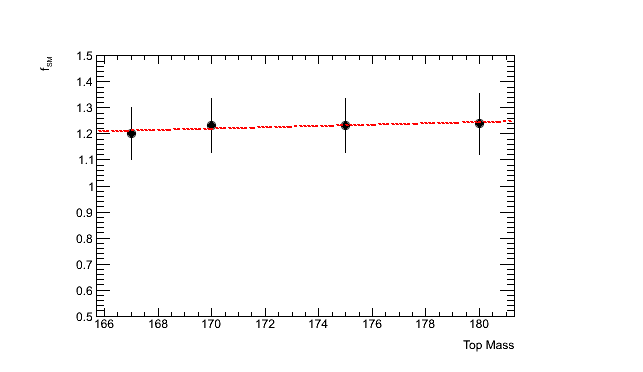
\includegraphics[width = 75mm]{f/delta_phi10_emu_TopMassTest}
	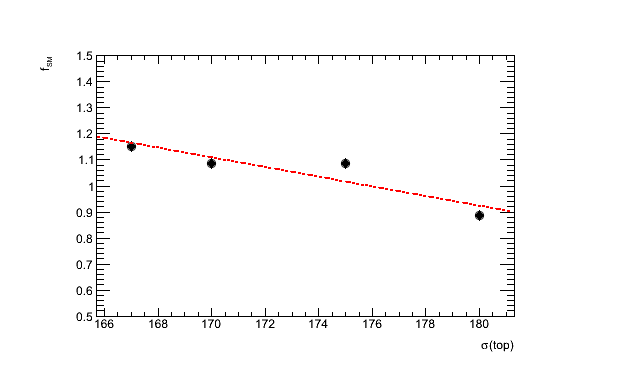
\includegraphics[width = 75mm]{f/delta_phi10_emu_TopMass_XsecTest}
	\end{center}
       \caption{Linear fit for $f_{SM}$ as a function of the top mass in the template for the \emu channel for the $\Delta\phi$ variable. The gradient of the fitted first order polynomial is 0.0025, showling a small dependence on the extracted $f_{SM}$ on the input top mass.}	
        \label{fig:top_mass}
\end{figure}

\vspace{5mm}
\noindent
\textbf{Top width in uncorrelated sample:}\newline
Due to the method used to generate the uncorrelated sample, the top and anti-top quarks were treated as on-shell particles by the generator and therefore did not include an intrinsic width. In order to estimate the effect of this, if any, the degree of spin correlation in the SM sample was investigated as a function of top mass. No correlation is observed between the top mass and the spin correlation and we exclude this as a source of systematic uncertainty .

\begin{figure}[hbtp]
	\begin{center}
	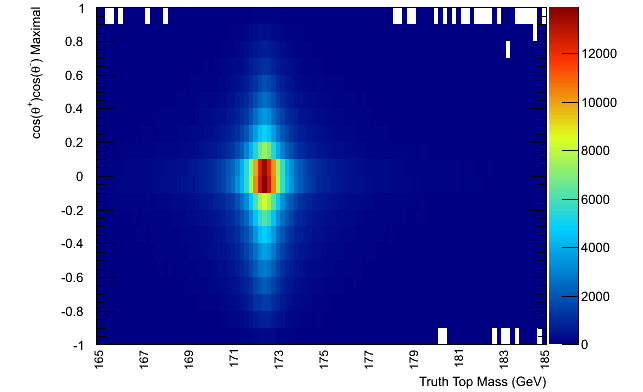
\includegraphics[width = 75mm]{f/TopCorrelationMass}
%	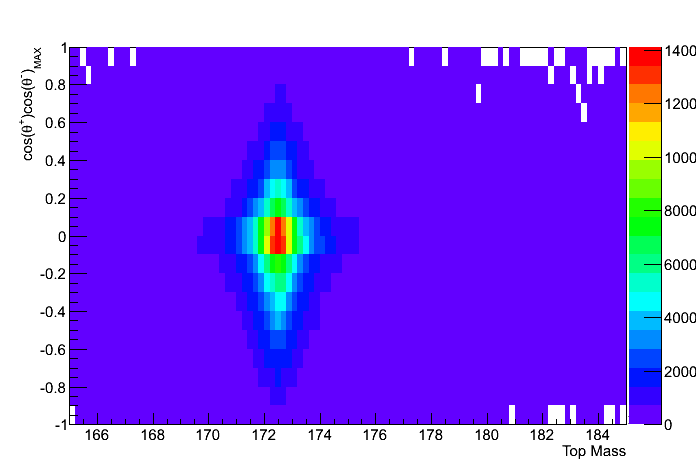
\includegraphics[width = 75mm]{f/AntiTopCorrelationMass}
	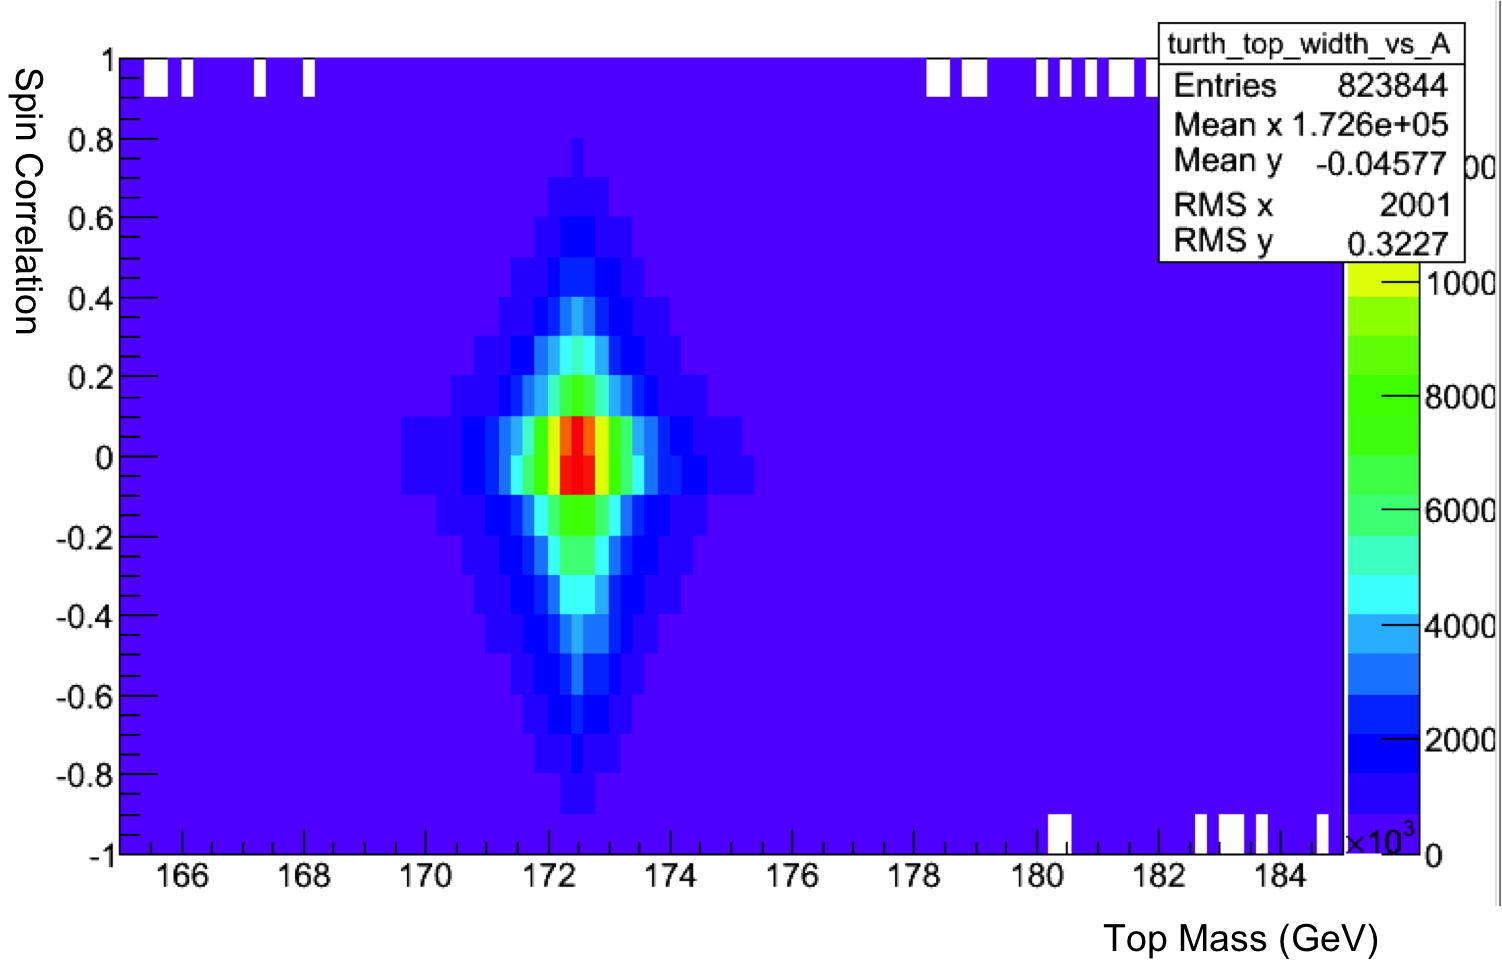
\includegraphics[width = 75mm]{f/Spinvstopwidth}
	\end{center}
        \caption{Correlation between top quark mass and the $\cos(\theta^+)\cos(\theta^-)_{MAXIMAL}$ variable \emph{(left)} and spin correlation \emph{(right)}}.	
        \label{fig:top_width}
\end{figure}